\documentclass[10pt]{beamer}

\mode<presentation>
{
  \usetheme{Frankfurt}
  \usecolortheme{rose}
  \setbeamercovered{transparent}
  \setbeamertemplate{footline}{}  
}

\usepackage[english]{babel}
\usepackage[latin1]{inputenc}

\usepackage{times}
\usepackage[T1]{fontenc}
\usepackage{graphicx}
\usepackage{tikz}
\usetikzlibrary{arrows,shapes}
\usepackage{amsmath}
\usepackage{verbatim}
\usepackage{xcolor}
\definecolor{dark}{rgb}{0.4,0.15,0.15}
\definecolor{dark-blue}{rgb}{0.15,0.15,0.4}
\definecolor{medium-blue}{rgb}{0,0,0.5}
\hypersetup{
    colorlinks, linkcolor={black},
    citecolor={dark-blue}, urlcolor={medium-blue}
}


\title%[\pgfuseimage{department-logo}]
{PW-Teleman\\
Tutorial }
\author[shortname]{author
 }
\institute[shortinst]{institute}


\vspace{0.5cm}




\vspace{1cm}

\titlegraphic{
\includegraphics[width=5cm]{teleman-logo}}


%%%%%%%%%%%%%%%%%%%%%%%%%%%%%%%%%%%%%%%%%%%%%%%%%%%%

\begin{document}
\tikzstyle{every picture}+=[remember picture]

\begin{frame}
\titlepage{}
\end{frame}
%%%%%%%%%%%%%%%%%%%%%%%%%%%%%%%%%%%%%%%%%%%%%%%%%%%%%
%%%%%%%%%%%%%%%%%%%%%%%%%%%%%%%%%%%%%%%%%%%%%%%%%%%%%

\begin{frame}
\begin{enumerate}
\item Useful information about PW-Teleman:\\
\vspace*{0.2cm}
{\tt prompt > cd \$pw-teleman\_dev-all\_201409/doc}\\
\vspace*{0.2cm}
{\tt prompt > ls}\\
\vspace*{0.4cm}

\begin{tabular}{ll}
\vspace*{0.2cm}
{\tt explain-init.pdf}& \footnotesize{\textcolor{red}{installation and description of the input files}}\\
\vspace*{0.2cm}
{\tt openmp\_explain.txt} & \footnotesize{\textcolor{red}{instructions for the OpenMP version of the 3D code}}\\
\vspace*{0.2cm}
{\tt modif\_dev-pgr.txt} &\footnotesize{\textcolor{red}{changes in the branch 'dev-pgr'}}\\
\vspace*{0.2cm}
{\tt FFT.txt} & \footnotesize{\textcolor{red}{modified make commands}}\\
\vspace*{0.2cm}
{\tt ase-pwteleman.txt} & \footnotesize{\textcolor{red}{coupling of the PWTELEMAN code with ASE}}\\
\end{tabular}
\vspace*{0.2cm}
\item Several examples that illustrate some of the features implemented in the code:\\
\vspace*{0.2cm}
{\tt prompt > cd \$pw-teleman\_dev-all\_201409/doc}
\end{enumerate}
\end{frame}

%%%%%%%%%%%%%%%%%%%%%%%%%%%%%%%%%%%%%%%%%%%%%%%%%%%%%
%%%%%%%%%%%%%%%%%%%%%%%%%%%%%%%%%%%%%%%%%%%%%%%%%%%%%

\begin{frame}
\frametitle{Before you start the calculations}
\begin{enumerate}  
\item Just go in the pwteleman directory and enter {\tt source ./install_pwteleman} and follow the instructions
\item The only prerequisite is a working {\tt gfortran} in your path (type  {\tt sudo apt-get install gfortran} if you have root on Linux)
\item Enter {\tt source ./install_pwteleman d } for gfortran compilation with debug options 
\item  {\tt source ./install_pwteleman a }for all possible compilations, if you have Intel Fortran Compiler and NVCC 

\item   {\tt source ./install_pwteleman t }to test your results and cross-correlate them against reference results  (quite long) 
\item  At any time you can try {\tt code/source_f90/regressionmatrix} to measure the change in your results vs reference results 
\item   {\tt source ./install_pwteleman i } for GPU compilations only (if you have Intel Fortran and NVCC) 
\item if it fails  to {\tt source\_f90} directory :\\
\vspace*{0.2cm}
{\tt cd pw-teleman\_dev-all\_20131009/code/source\_f90/
}\\
\vspace*{0.2cm}
Before compilation, you might want to update some settings,\\ for detailed explanations see {\tt openmp\_explain.txt}.
\vspace*{0.2cm}
\item To use environment modules for compiling or running a code you have to load a particular module\\
\vspace*{0.2cm}
{\tt module load <module name>}
\vspace*{0.2cm}
\item For GPUs see {\tt gpu\_explain.txt}).
\item Execute {\tt make} command which you can modify in several ways (see {\tt openmp\_explain.txt}). In our example we compile the code with FFTW functions using parallelization for wavefunctions:\\
\vspace*{0.2cm}
\vspace*{0.2cm}
{\tt ./make.sh 1 fftw} 
\vspace*{0.2cm}
\item The executable will be copied to the working
 directory which is one level below the sub-directory {\tt source\_f90}. The file called {\tt pwteleman.par} is
 the new executable.
\end{enumerate} 
 
 %\includegraphics[width=4.5cm]<1->{fig/magh}

   
\end{frame}

%%%%%%%%%%%%%%%%%%%%%%%%%%%%%%%%%%%%%%%%%%%%%%%%%%%%%
\begin{frame}
\frametitle{Jellium model for Na8 - Real Time TDDFT}
\begin{enumerate}
\item Go the {\tt na8-jel} directory\\
\vspace*{0.2cm}
{\tt cd pw-teleman\_dev-all\_20131009/samples/na8-jel}\\
\vspace*{0.2cm}
you should see following files:\\
\vspace*{0.2cm}
\begin{tabular}{ll}
{\tt for005.na8-jel} &{\scriptsize{\textcolor{red}{general input for settings, static and dynamics}}}\\
{\tt for005}  &{\scriptsize{\textcolor{red}{defines the qualifier na8-jel for the other {\tt for005} files}}}\\
\end{tabular}
\vspace*{0.4cm}


\item Open and read the sample file {\tt for005.na8-jel}, there are three namelists:\\
\vspace*{0.4cm}
\begin{tabular}{ll}
 {\tt \&GLOBAL} & {\scriptsize{\textcolor{red}{choice of the system, initialization of wave functions, convergence issues}}}\\
{\tt \&DYNAMIC}&{\scriptsize{\textcolor{red}{numerical and physical parameters for statics and dynamics, }}}\\
&{\scriptsize{\textcolor{red}{way of excitation, flags for observables}}}\\
 {\tt \&SURFACE}&\\
 \vspace*{0.2cm}
\end{tabular}
In file {\tt openmp\_explain.txt} you can find complete description of the parameters used in the input. 
\end{enumerate}
\end{frame}
%%%%%%%%%%%%%%%%%%%%%%%%%%%%%%%%%%%%%%%%%%%%%%%%%%%%%
%%%%%%%%%%%%%%%%%%%%%%%%%%%%%%%%%%%%%%%%%%%%%%%%%%%%%

\begin{frame}
\frametitle{ }
\begin{enumerate}  
\item  Run the code using mpirun command or mpiexec depending on your installation (or include it in a batch submission):\\
\vspace*{0.2cm}
{\tt mpirun [mpirun\_options] ../../code/pwteleman.par}\\
\vspace*{0.2cm}
e.g.:\\
\vspace*{0.2cm}
{\tt mpirun -np 8 ../../code/pwteleman.par}\\
\vspace*{0.2cm}
(using 8 processors to run on)
\vspace*{0.4cm}
\item You will get several output files, e.g.:\\
\vspace*{0.2cm}
\begin{tabular}{ll}
\vspace*{0.1cm}
{\tt for006.0na8-jel} & {\small{\textcolor{red}{main output}}}\\
\vspace*{0.1cm}
{\tt energies.na8-jel} &{\small{\textcolor{red}{binding energy}}}\\
\vspace*{0.1cm}
{\tt pdip.na8-jel}& {\small{\textcolor{red}{dipole moments}}}\\
\vspace*{0.1cm}
{\tt infosp.na8-jel} & {\small{\textcolor{red}{dynamical informations}}}\\
\vspace*{0.1cm}
{\tt pquad.na8-jel} & {\small{\textcolor{red}{quadripol moments}}}\\
\vspace*{0.1cm}
{\tt penergies.na8-jel} & {\small{\textcolor{red}{energy informations}}}\\
\end{tabular}
\end{enumerate} 
 
 %\includegraphics[width=4.5cm]<1->{fig/magh}

   
\end{frame}

%%%%%%%%%%%%%%%%%%%%%%%%%%%%%%%%%%%%%%%%%%%%%%%%%%%%%
%%%%%%%%%%%%%%%%%%%%%%%%%%%%%%%%%%%%%%%%%%%%%%%%%%%%%

\begin{frame}
\frametitle{Let's plot the results - Dipole moment}
To plot time vs dipole moment, copy {\tt pdip.na8-jel} into {\tt pdip}:\\
\vspace*{0.2cm}
{\tt cp} {\tt pdip.na8-jel} {\tt pdip}\\
\vspace*{0.2cm}
Open {\tt pdip} and remove six first lines to get the readable format to gnuplot, then:\\
\vspace*{0.2cm}
{\tt gnuplot> set xlabel 'Time step'\\
gnuplot> set ylabel 'Dipole moment'\\
gnuplot> unset key \\
gnuplot> plot './pdip'  w l}\\


   
\end{frame}



%%%%%%%%%%%%%%%%%%%%%%%%%%%%%%%%%%%%%%%%%%%%%%%%%%%%%
%%%%%%%%%%%%%%%%%%%%%%%%%%%%%%%%%%%%%%%%%%%%%%%%%%%%%

\begin{frame}
\frametitle{Let's plot the results - Dipole moment}

\centering
 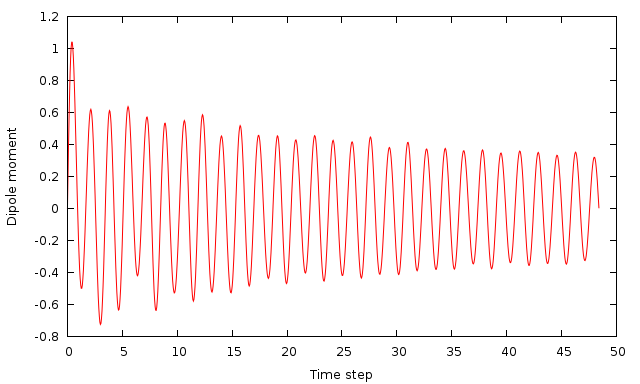
\includegraphics[width=10cm]{fig/dipole}

   
\end{frame}

%%%%%%%%%%%%%%%%%%%%%%%%%%%%%%%%%%%%%%%%%%%%%%%%%%%%%
%%%%%%%%%%%%%%%%%%%%%%%%%%%%%%%%%%%%%%%%%%%%%%%%%%%%%

\begin{frame}
\frametitle{Let's plot the results- Absorption spectra}
You need to increase {\tt ismax}  and {\tt itmax}  to larger values in file  {\tt for005.na8jel  } 
and rerun the code, maybe  in batch mode 
To obtain the data for absorption spectra you need to compile and run a {\tt spectr2.F90} code:\\
\vspace*{0.2cm}
{\tt cd pw-teleman\_dev-all\_20131009/code/source\_aux}\\
\vspace*{0.1cm}
{\tt gfortran spectr2.F90 -o spectr}\\
\vspace*{0.1cm}
{\tt ../../code/source\_aux/spectr < pdip.na8-jel > spectra}\\
\vspace*{0.2cm}
Data you need to plot absorption spectra will be collected in {\tt spectra}, make the file readable to gnuplot and then:\\
\vspace*{0.2cm}

{\tt gnuplot> set xlabel 'Energy [eV]'\\
gnuplot> set ylabel 'oscillator strength'\\
gnuplot> unset key \\
gnuplot>  set xrange [0:5]\\
gnuplot>  plot './spectra' u 2:3 w l
}\\
  
\end{frame}



%%%%%%%%%%%%%%%%%%%%%%%%%%%%%%%%%%%%%%%%%%%%%%%%%%%%%
%%%%%%%%%%%%%%%%%%%%%%%%%%%%%%%%%%%%%%%%%%%%%%%%%%%%%

\begin{frame}
\frametitle{Let's plot the results - Absorption spectra}

\centering
 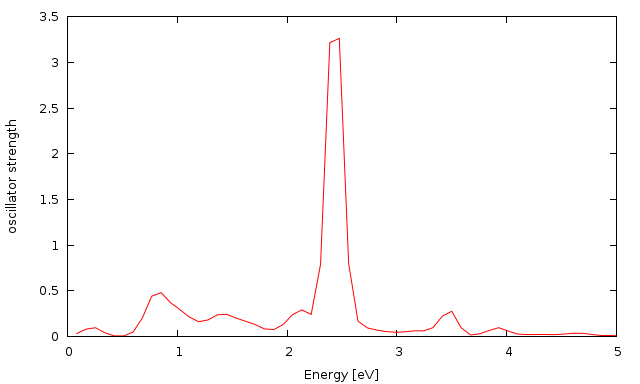
\includegraphics[width=11cm]{fig/spectr}



   
\end{frame}



%%%%%%%%%%%%%%%%%%%%%%%%%%%%%%%%%%%%%%%%%%%%%%%%%%%%%
%%%%%%%%%%%%%%%%%%%%%%%%%%%%%%%%%%%%%%%%%%%%%%%%%%%%%
\begin{frame}
\frametitle{Oscillatory motion of diatomic molecule - hydrogen}
\begin{enumerate}
\item Go the {\tt H2} directory\\
\vspace*{0.2cm}
{\tt cd pw-teleman\_dev-all\_20131009/samples_py/H2}\\
\vspace*{0.2cm}
you should see following files:\\
\vspace*{0.2cm}
\begin{tabular}{lll}
{\tt for005.H2} &{\scriptsize{\textcolor{red}{general input for settings, static and dynamics}}}\\
{\tt for005}  &{\scriptsize{\textcolor{red}{defines the qualifier na8-jel for the other {\tt for005} files}}}\\
{\tt for005ion.H2} &{\scriptsize{\textcolor{red}{ionic configuration of cluster}}}\\
\end{tabular}
\vspace*{0.4cm}


\item Open and read the sample file {\tt for005.H2}, there are three namelists:\\
\vspace*{0.4cm}
\begin{tabular}{ll}
 {\tt \&GLOBAL} & {\scriptsize{\textcolor{red}{choice of the system, initialization of wave functions, convergence issues}}}\\
{\tt \&DYNAMIC}&{\scriptsize{\textcolor{red}{numerical and physical parameters for statics and dynamics, }}}\\
&{\scriptsize{\textcolor{red}{way of excitation, flags for observables}}}\\
 {\tt \&PERIO}&{\scriptsize{\textcolor{red}{needed when  {\tt ipsptype=1}}}}\\
 \vspace*{0.2cm}
\end{tabular}
In file {\tt openmp\_explain.txt} you can find complete description of the parameters used in the input. 
You can alternatively input  {\tt ipsptype=3} or  {\tt ipsptype=4} in which case the pseudopotential
parameters are read from file {\tt goed.asci} and {\tt periodic}  which you need in the present directory.
You can alternatively use  {\tt nclust=0} in which case the total number of electrons is automatically computed.
(see anilin example)
If you set a negative {\tt dx,dy,dz} the optimal value will be determinated from the pseudopotential file
and a recommanded {\tt kxbox, kybox,kzbox} will be given and written to file {\tt nx}. The program then quits. In the
next run, this value will be used.

\end{enumerate}
\end{frame}
%%%%%%%%%%%%%%%%%%%%%%%%%%%%%%%%%%%%%%%%%%%%%%%%%%%%%
%%%%%%%%%%%%%%%%%%%%%%%%%%%%%%%%%%%%%%%%%%%%%%%%%%%%%
\begin{frame}

Now open open sample file {\tt for005ion.H2},  you will see two lines:

  \vspace{1cm}     
  
~
    \tikz[baseline]{
        \node[fill=blue!20,anchor=base] (xyz1)
    {{\tt\scriptsize{0.09597562751811~0.09597562746044  -0.89554425290261~}}};
    }
    \tikz[baseline]{
        \node[fill=red!20,anchor=base] (h1)
    {{\tt \scriptsize{1}}};
    }
    \tikz[baseline]{
        \node[fill=green!20,anchor=base] (A1)
    {{\tt\scriptsize{xyz}}};
    }
    \tikz[baseline]{
        \node[fill=yellow!20,anchor=base] (V1)
    {{\tt\scriptsize{1.0}}};
    }
    \tikz[baseline]{
        \node[fill=magenta!20,anchor=base] (beta1)
    {{\tt\scriptsize{-1~}}};
    }

      
~
    \tikz[baseline]{
        \node[fill=blue!20,anchor=base] (xyz1)
    {{\tt\scriptsize{0.09597905125029~0.09597905333623~ 0.89609579462877}}};
    }
    \tikz[baseline]{
        \node[fill=red!20,anchor=base] (h1)
    {{\tt\scriptsize{1}}};
    }
    \tikz[baseline]{
        \node[fill=green!20,anchor=base] (A1)
    {{\tt\scriptsize{xyz}}};
    }
    \tikz[baseline]{
        \node[fill=yellow!20,anchor=base] (V1)
    {{\tt\scriptsize{1.0}}};
    }
    \tikz[baseline]{
        \node[fill=magenta!20,anchor=base] (b1)
    {{\tt\scriptsize{1~~}}};
    }
    
 \vspace{1cm}   
 where: 
 
\begin{itemize}
    \item x,y,z coordinates
        \tikz \node [coordinate] (xyz2) {};
    \item number of element in periodic system
        \tikz \node [coordinate] (h2) {};
    \item only {\tt init\_lcao=1}: ordering of nodes in repeat initialization at this ion
        \tikz \node [coordinate] (A2) {};
    \item only {\tt init\_lcao=1}: radius of initial Gaussian at this ion
        \tikz \node [coordinate] (V2) {};
    \item only {\tt init\_lcao=1}: starting spin for initialization at this ion
        \tikz \node [coordinate] (b2) {};
\end{itemize}
\begin{tikzpicture}[overlay]
        \path[->,blue] (xyz2) edge [bend right] (xyz1);
        \path[->,red] (h2)      edge [bend right] (h1);
        \path[->,green] (A2)      edge [bend right] (A1);
        \path[->,yellow] (V2)      edge [bend right] (V1);
        \path[->,magenta] (b2)   edge [bend right] (b1);
\end{tikzpicture}
\end{frame}
%%%%%%%%%%%%%%%%%%%%%%%%%%%%%%%%%%%%%%%%%%%%%%%%%%%%%

\begin{frame}
\frametitle{ }
In case when the number of the wavefunctions is too little the calculations might fail, thus, in this example we will run the code in serial. \\
\vspace*{0.4cm}
\begin{enumerate} 
\item Go to {\tt source\_f90} directory:\\
\vspace*{0.2cm}
{\tt cd ..}\\
{\tt cd ..}\\
{\tt cd code/source\_f90/}\\
\vspace*{0.2cm}
\item Execute {\tt make} command and compile the code with FFTW functions to produce serial code:\\
\vspace*{0.2cm}
{\tt ./make.sh 0 fftw}\\
\vspace*{0.2cm}
The new executable called {\tt pwteleman.seq} will be in the directory {\tt code} which is one level below the sub-directory {\tt source\_f90}\\
\vspace*{0.4cm}
\item  Go back to the {\tt H2} directory and run the code:\\
\vspace*{0.2cm}
{\tt ../../code/pwteleman.seq}\\
\vspace*{0.2cm}

\end{enumerate} 
 
 %\includegraphics[width=4.5cm]<1->{fig/magh}

   
\end{frame}


%%%%%%%%%%%%%%%%%%%%%%%%%%%%%%%%%%%%%%%%%%%%%%%%%%%%%

\begin{frame}
\begin{enumerate}
\item You will get several output files, e.g.:\\
\vspace*{0.2cm}
\begin{tabular}{ll}
\vspace*{0.1cm}
{\tt for006.0H2} & {\small{\textcolor{red}{main output}}}\\
\vspace*{0.1cm}
{\tt energies.H2} &{\small{\textcolor{red}{binding energy}}}\\
\vspace*{0.1cm}
{\tt pdip.H2}& {\small{\textcolor{red}{dipole moments}}}\\
\vspace*{0.1cm}
{\tt infosp.H2} & {\small{\textcolor{red}{dynamical informations}}}\\
\vspace*{0.1cm}
{\tt pvelion.H2} & {\small{\textcolor{red}{ionic velocities}}}\\
\vspace*{0.1cm}
{\tt penergies.H2} & {\small{\textcolor{red}{energy informations}}}\\
\vspace*{0.1cm}
{\tt pposion.H2} & {\small{\textcolor{red}{ionic positions}}}\\
\end{tabular}
\vspace*{0.2cm}
\item The last one {\tt pposion.H2} will be needed to estimate the oscillation period of diatomic hydrogen. \\
\vspace*{0.2cm}
\item Use plotting software to draw   'Positions vs Time' graph, \\e.g. with gnuplot:\\
\vspace*{0.1cm}
{\tt gnuplot> set ylabel 'Positions'}\\
{\tt gnuplot> set xlabel 'Time'}\\
{\tt gnuplot> set xrange [0:20]}\\
{\tt gnuplot> unset key}\\
{\tt gnuplot> plot './pposion.H2'u 1:5 w d}\\
\end{enumerate}
\end{frame}



%%%%%%%%%%%%%%%%%%%%%%%%%%%%%%%%%%%%%%%%%%%%%%%%%%%%%

%%%%%%%%%%%%%%%%%%%%%%%%%%%%%%%%%%%%%%%%%%%%%%%%%%%%%

\begin{frame}
This will show following graph:\\

\centering
 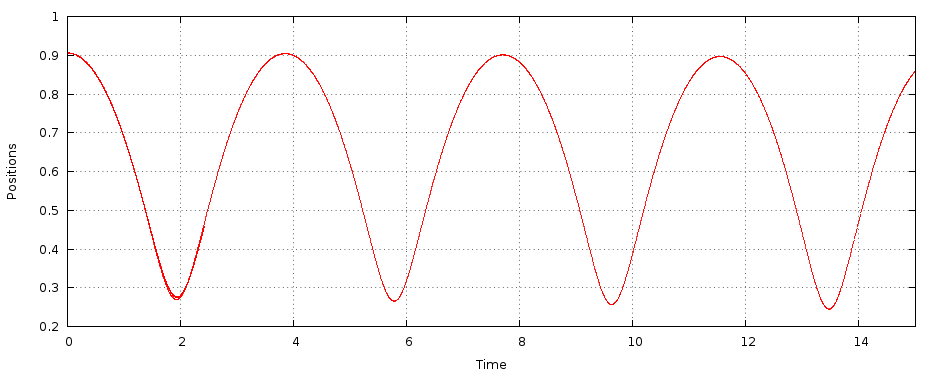
\includegraphics[width=11.5cm]{fig/period}

From closer inspection you can see that the corresponding period of the oscillation is 4 units.

\end{frame}



%%%%%%%%%%%%%%%%%%%%%%%%%%%%%%%%%%%%%%%%%%%%%%%%%%%%%
%%%%%%%%%%%%%%%%%%%%%%%%%%%%%%%%%%%%%%%%%%%%%%%%%%%%%

\begin{frame}
\frametitle{Coupling of the PWTELEMAN code with ASE}

\begin{block}{}
   \href{https://wiki.fysik.dtu.dk/ase/overview.html}{ASE} is an Atomistic Simulation Environment written in the \href{http://www.python.org/}{Python} programming language with the aim of setting up, steering, and analyzing atomistic simulations .\\
    The coupling of the PWTELEMAN code with ASE  is still in progress.
   \end{block}
   \vspace*{1.2cm}

\begin{columns}
  \begin{column}{0.5\textwidth}
  Useful informations about ASE:\\
     \vspace*{0.2cm}
Overview \href{https://wiki.fysik.dtu.dk/ase/overview.html}{\beamerbutton{click!}}\\
What is Phyton? \href{https://wiki.fysik.dtu.dk/ase/python.html#python-info}{\beamerbutton{click!}}\\
ASE and Phyton tutorials \href{https://wiki.fysik.dtu.dk/ase/tutorials/tutorials.html}{\beamerbutton{click!}}\\
Documentation \href{https://wiki.fysik.dtu.dk/ase/ase/ase.html}{\beamerbutton{click!}}\\
  \end{column}
  \begin{column}{0.5\textwidth}
  \centering
 
\includegraphics[width=5.5cm]{fig/co}   
  \end{column}
\end{columns}

\end{frame}


%%%%%%%%%%%%%%%%%%%%%%%%%%%%%%%%%%%%%%%%%%%%%%%%%%%%%
%%%%%%%%%%%%%%%%%%%%%%%%%%%%%%%%%%%%%%%%%%%%%%%%%%%%%

\begin{frame}
\frametitle{PWTELEMAN-ASE : An example using Na}
\begin{enumerate}

\item \small{First thing, you need to install ASE: \href{https://wiki.fysik.dtu.dk/ase/download.html}{https://wiki.fysik.dtu.dk/ase/download.html}
\item \small{Run the install script in order to get paths correcly, or look into it }
\item \small{{\tt source ./install_pwteleman}
     \vspace*{0.2cm}
     
\item Then, go to {\tt Na} directory:}\\
\small{{\tt cd pw-teleman\_dev-all\_20131009/code/source\_py/Na_ase}}\\
You should see the  following files : \\
{\tt na.py}
\vspace*{0.2cm}


\item \small{Place the file {\tt na.py} in your working directory}
\vspace*{0.2cm}

\item Run the python script with the following command : }\\
{\tt python na.py}
\item If it fails, edit the  {\tt pwteleman\_SCRIPT} environment variable as follow :\\ 
\footnotesize{{\tt 
export pwteleman\_SCRIPT=\textasciitilde/pwtelemanscript.py}}
\vspace*{0.2cm}

\item \small{In the file {\tt pwtelemanscript.py}, replace the location of PWTELEMAN code by your actual path (line 3)
\vspace*{0.2cm}

\end{enumerate}

\small{ASE will automatically generate the input files for the PWTELEMAN code (the for005* files) and then run the code itself. }

\end{frame}



%%%%%%%%%%%%%%%%%%%%%%%%%%%%%%%%%%%%%%%%%%%%%%%%%%%%%
\begin{frame}
\frametitle{ Relaxation of ionic coordinates:\\
PWTELEMAN-ASE coupling example of H2}
\begin{enumerate}
\item \small{Create a sub-directory {\tt H2py} for example in {\tt samples}:\\
{\tt cd pwteleman/pw-teleman\_dev-all\_20131009/samples/}
{\tt mkdir H2py}
{\tt cd H2py}\\
{\tt cp ../../code/Python\_ASE/Na/na.py .}\\
\end{enumerate}
\end{frame}
%%%%%%%%%%%%%%%%%%%%%%%%%%%%%%%%%%%%%%%%%%%%%%%%%%%%%

\begin{frame}
Now prepare input with coordinates in \href{http://openbabel.org/wiki/XYZ\_(format)}{XYZ} chemical file format.\\
The format is as follows:\\
~\\
{\tt <# of atoms>\\
comment line\\
atom1 x-coord1 y-coord1 z-coord1\\
atom2 x-coord2 y-coord2 z-coord2\\
...\\
atomN x-coordN y-coordN z-coordN}\\
~\\
For example:\\
{\tt 2\\
~~\\
H	0.0	0.0	-1.0\\
H	0.0	0.0	1.0\\}
~\\
Call the file {\tt H2.xyz}
\end{frame}



%%%%%%%%%%%%%%%%%%%%%%%%%%%%%%%%%%%%%%%%%%%%%%%%%%%%%

%%%%%%%%%%%%%%%%%%%%%%%%%%%%%%%%%%%%%%%%%%%%%%%%%%%%%

\begin{frame}
Then you should rename the file {\tt na.py}\\
{\tt mv na.py h2.py}\\
and adapt it to the needs of this example of H2 using e.g. gedit:\\
{\tt gedit h2.py}\\
~\\
\small{{\tt h2=read(\textcolor{magenta}{'h2.xyz'})\\
\textcolor{blue}{#from ase.calculators.pwteleman import pwteleman}\\
\textcolor{magenta}{from} ase.calculators.pwtelemandynr \textcolor{magenta}{import} pwtelemandynr\\
~\\
h2.set\_calculator(pwtelemandynr(isurf=\textcolor{magenta}{0},dx=\textcolor{magenta}{0.2354},dy=\textcolor{magenta}{0.2354},\\dz=\textcolor{magenta}{0.2354},
kxbox=\textcolor{magenta}{24},kybox=\textcolor{magenta}{24},kzbox=\textcolor{magenta}{48},nspdw=\textcolor{magenta}{1},init\_lcao=1,ismax=20,\\ modecalc=\textcolor{magenta}{'static'}))\\
e = h2.get\_potential\_energy()\\
print e\\
traj=PickleTrajectory(\textcolor{magenta}{'h2.traj'},\textcolor{magenta}{'w'})\\
dyn=QuasiNewton(h2).run(fmax=\textcolor{magenta}{0.0001})\\
e = h2.get\_potential\_energy()\\
print e-\textcolor{magenta}{4}*\textcolor{magenta}{13.6}}}
\end{frame}



%%%%%%%%%%%%%%%%%%%%%%%%%%%%%%%%%%%%%%%%%%%%%%%%%%%%%%%%%%%%%%%%%%%%%%%%%%%%%%%%%%%%%%%%%%%%%%%%%%%%%%%%%%

\begin{frame}
The last step is to run a calculations:\\
\hspace*{0.2cm}

{\tt python h2.py}\\
\hspace*{0.2cm}

All for005* files will be generated automatically by ASE and then the code will run itself. \\
In file {\tt for005ion.pwteleman} you can find the final coordinates after relaxation. 

\end{frame}

%%%%%%%%%%%%%%%%%%%%%%%%%%%%%%%%%%%%%%%%%%%%%%%%%%%%%%%%%%%%%%%%%%%%%%%%%%%%%%%%%%%%%%%%%%%%%%%%%%%%%%%%%%

\begin{frame}
\frametitle{Absorption spectra of free cluster Na9+}
\begin{enumerate}
\item Go the {\tt na9} directory\\
\vspace*{0.2cm}
{\tt cd pw-teleman\_dev-all\_20131009/samples/na9}\\
\vspace*{0.2cm}
you should see following files:\\
\vspace*{0.2cm}
\begin{tabular}{ll}
{\tt for005.na9} &{\scriptsize{\textcolor{red}{general input for settings, static and dynamics}}}\\
{\tt for005}  &{\scriptsize{\textcolor{red}{defines the qualifier na9 for the other {\tt for005} files}}}\\
{\tt for005ion.na9}  &{\scriptsize{\textcolor{red}{ionic configuration of cluster}}}\\
\end{tabular}
\vspace*{0.4cm}


\item Open and read the sample file {\tt for005.na9}, the number of electrons ({\tt nclust}) should be set to {\tt 8} and the numer of cluster ions ({\tt nion}) to {\tt 9}. 

\item Run the code:

{\tt ../../code/pwteleman.seq}

\item To obtain the data for absorption spectra run a {\tt spectr2.F90} code:

\small{{\tt ../../code/source\_aux/spectr < pdip.na9 > spectra}}
\end{enumerate}

\end{frame}
%%%%%%%%%%%%%%%%%%%%%%%%%%%%%%%%%%%%%%%%%%%%%%%%%%%%%
\begin{frame}

\small{Necessary data to plot absorption spectra is collected in {\tt spectra}, make the file readable to gnuplot and then:\\}
\vspace*{0.2cm}

\small{{\tt gnuplot> set xlabel 'Energy [eV]'\\
gnuplot> set ylabel 'Oscillator strength'\\
gnuplot> unset key \\
gnuplot>  set xrange [0:10]\\
gnuplot>  plot './spectra' u 2:5 w l
}}\\

\centering
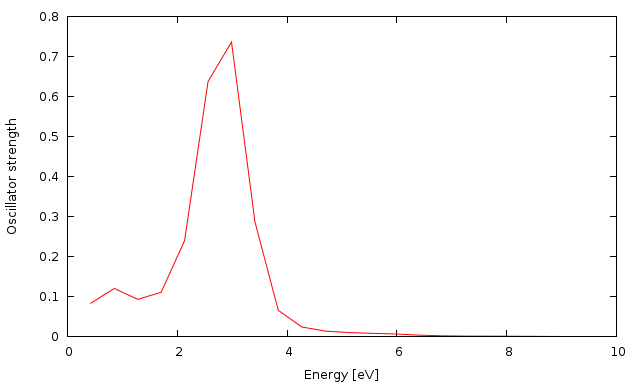
\includegraphics[width=8.5cm]{fig/spectrana9} 

\end{frame}

%%%%%%%%%%%%%%%%%%%%%%%%%%%%%%%%%%%%%%%%%%%%%%%%%%%%
%%%%%%%%%%%%%%%%%%%%%%%%%%%%%%%%%%%%%%%%%%%%%%%%%%%%%
\begin{frame}

\small{To plot time vs dipole moment copy {\tt pdip.na9} to {\tt pdip} and make it readable to gnuplot, then:\\}
\vspace*{0.2cm}

\small{{\tt gnuplot> set xlabel 'Time step'\\
gnuplot> set ylabel 'Dipole moment'\\
gnuplot> unset key \\
gnuplot>  set xrange [0:10]\\
gnuplot>  plot './pdip'  w l
}}\\

\centering
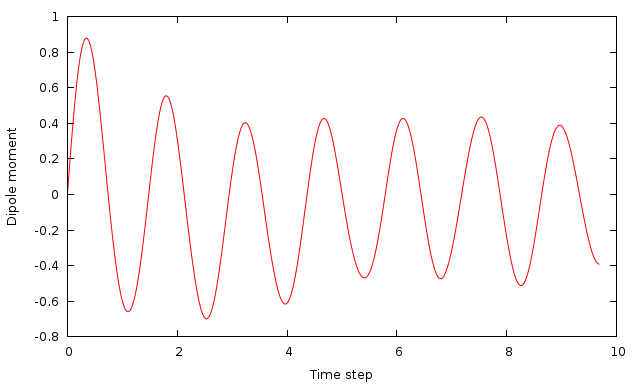
\includegraphics[width=8.5cm]{fig/dipolena9} 

\end{frame}

%%%%%%%%%%%%%%%%%%%%%%%%%%%%%%%%%%%%%%%%%%%%%%%%%%%%
\begin{frame}
\frametitle{Jellium model for Na9+}
\begin{enumerate}
\item Go the {\tt na9-jel} directory\\
\vspace*{0.2cm}
{\tt cd pw-teleman\_dev-all\_20131009/samples/na8-jel}\\
\vspace*{0.2cm}
you should see following files:\\
\vspace*{0.2cm}
\begin{tabular}{ll}
{\tt for005.na9-jel} &{\scriptsize{\textcolor{red}{general input for settings, static and dynamics}}}\\
{\tt for005}  &{\scriptsize{\textcolor{red}{defines the qualifier na9-jel for the other {\tt for005} files}}}\\
\end{tabular}
\vspace*{0.4cm}


\item In the sample file {\tt for005.na9-jel} you should notice that {\tt nion2} paremeter is set to {\tt 0} what stands for jellium background

\item To obtain the absorption spectra and dipole moment you should analogously follow the steps from the previous example. 
\end{enumerate}
\end{frame}
%%%%%%%%%%%%%%%%%%%%%%%%%%%%%%%%%%%%%%%%%%%%%%%%%%%%%
%%%%%%%%%%%%%%%%%%%%%%%%%%%%%%%%%%%%%%%%%%%%%%%%%%%%%%%%%%%%%%%%%%%%%%%%%%%%%%%%%%%%%%%%%%%%%%%%%%%%%%%%%%
%%%%%%%%%%%%%%%%%%%%%%%%%%%%%%%%%%%%%%%%%%%%%%%%%%%%%
\begin{frame}
\frametitle{Absorption spectra Na9+\\
Jellium model}

\centering
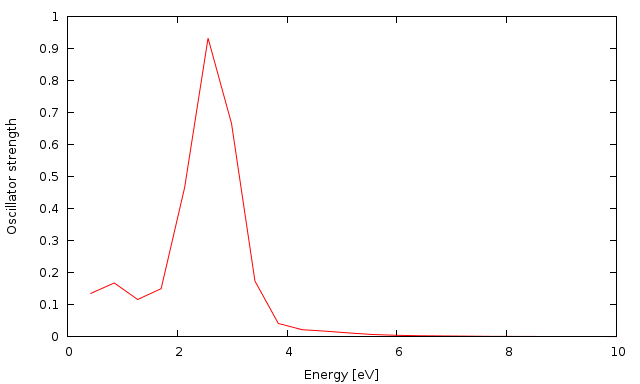
\includegraphics[width=11cm]{fig/spectrana9j} 

\end{frame}

%%%%%%%%%%%%%%%%%%%%%%%%%%%%%%%%%%%%%%%%%%%%%%%%%%%%
%%%%%%%%%%%%%%%%%%%%%%%%%%%%%%%%%%%%%%%%%%%%%%%%%%%%%
\begin{frame}
\frametitle{Dipole moment Na9+\\
Jellium model}

\centering
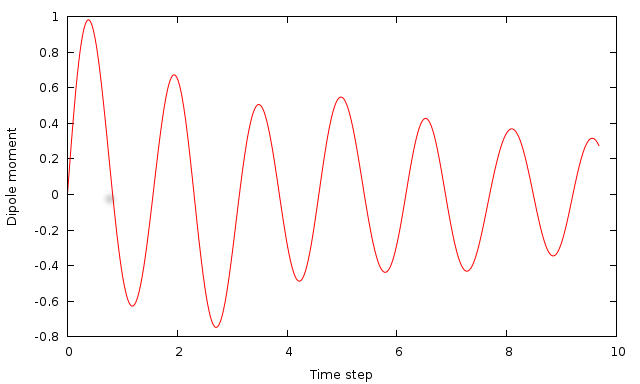
\includegraphics[width=11cm]{fig/dipolena9j} 

\end{frame}

%%%%%%%%%%%%%%%%%%%%%%%%%%%%%%%%%%%%%%%%%%%%%%%%%%%%
\begin{frame}
\frametitle{The investigation of energy conservation - H2}

To check the total energy of the molecule as a function of time follow the steps:

\begin{enumerate}
\item go to the {\tt H2} directory\\
{\tt cd pw-teleman\_dev-all\_20131009/samples_py/H2}
\item If you performed the previous calculations concerning H2, you should find there a file containing energy informations called {\tt penergies.H2}. 
\item To draw   'Positions vs Time' graph, you can use e.g. gnuplot:\\
\vspace*{0.1cm}
{\tt gnuplot> set ylabel 'Total energy'}\\
{\tt gnuplot> set xlabel 'Time step'}\\
{\tt gnuplot> unset key}\\
{\tt gnuplot> plot './penergies.H2' u 1:18 w l}\\


\end{enumerate}


\end{frame}



%%%%%%%%%%%%%%%%%%%%%%%%%%%%%%%%%%%%%%%%%%%%%%%%%%%%%%%%%%%%%%%%%%%%%%%%%%%%%%%%%%%%%%%%%%%%%%%%%%%%%%%%%%

\begin{frame}
\frametitle{The evolution of the energy over time.}

\centering
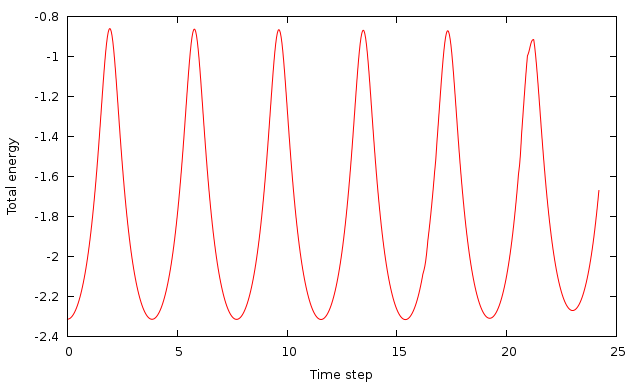
\includegraphics[width=11cm]{fig/enh2}
\end{frame}



%%%%%%%%%%%%%%%%%%%%%%%%%%%%%%%%%%%%%%%%%%%%%%%%%%%%%
%%%%%%%%%%%%%%%%%%%%%%%%%%%%%%%%%%%%%%%%%%%%%%%%%%%%%%%%%%%%%%%%%%%%%%%%%%%%%%%%%%%%%%%%%%%%%%%%%%%%%%%%%%
%%%%%%%%%%%%%%%%%%%%%%%%%%%%%%%%%%%%%%%%%%%%%%%%%%%%
\begin{frame}
\frametitle{Anilin - porphyrin spectrum}
\begin{enumerate}
\item Go the {\tt anilin} directory\\
\vspace*{0.2cm}
{\tt cd pw-teleman\_dev-all\_20131009/samples/anilin}\\
\vspace*{0.2cm}

\item In this case we use in {\tt anilin.py} the default settings of the ASE-PWTELEMAN calculator,
\item Grid spacing and total charge will be set automatically from the {\tt goed.asci} Goedecker pseudopotential file 
\item Default values have to be given for the 'static' mode of calculation 
\item Only the number of dynamic iterations and time steps/excitation have to be given for the 
'plasmon' mode
\item The same goes for the simplified porphyrin_mg molecule, with a much larger number of electrons

\end{frame}

\begin{frame}
~~
\end{frame}



%%%%%%%%%%%%%%%%%%%%%%%%%%%%%%%%%%%%%%%%%%%%%%%%%%%%%

\end{document}
